\subsection{Dimuon experiments and nuclear PDFs}

Most of our knowledge on the medium-modified PDFs come from DIS experiments. Although extensive and precise, 
these data are not able to independently investigate the nuclear effects on sea and valence quarks.  
Moreover, they do not discriminate between the different flavors participating in the reaction. Finally, 
they do not probe the nuclear gluon distributions. Additional studies of the effect of the medium on the 
PDFs can be provided by dedicated fixed-target dimuon production experiments. In the Drell-Yan mass region
 these experiments can be used to isolate  
valence and sea distributions as well as to separate the two light flavors of the quark PDFs. 
The unknown gluon distributions in nuclei can be accessed by analyzing the contributions to  
the charmonium production cross-sections. 
 
\subsubsection {Valence quark distributions and the EMC effect}
Only a few Drell-Yan experiments have investigated the medium modifications in nuclear targets. 
The Drell-Yan data from the E772 experiment~\cite{Alde:1990im} show no visible nuclear effects in 
the antishadowing domain, both E772 and E866 experiments~\cite{Vasilev:1999fa} are compatible 
with the DIS data in the onset of the shadowing region, Fig.~\ref{fig:drell-yan}.  An exploration of the medium effects for larger $x$ 
values was recently completed by the SeaQuest experiment~\cite{Arrington:2006} at Fermilab. 

\begin{center}
\begin{figure}[htb]
  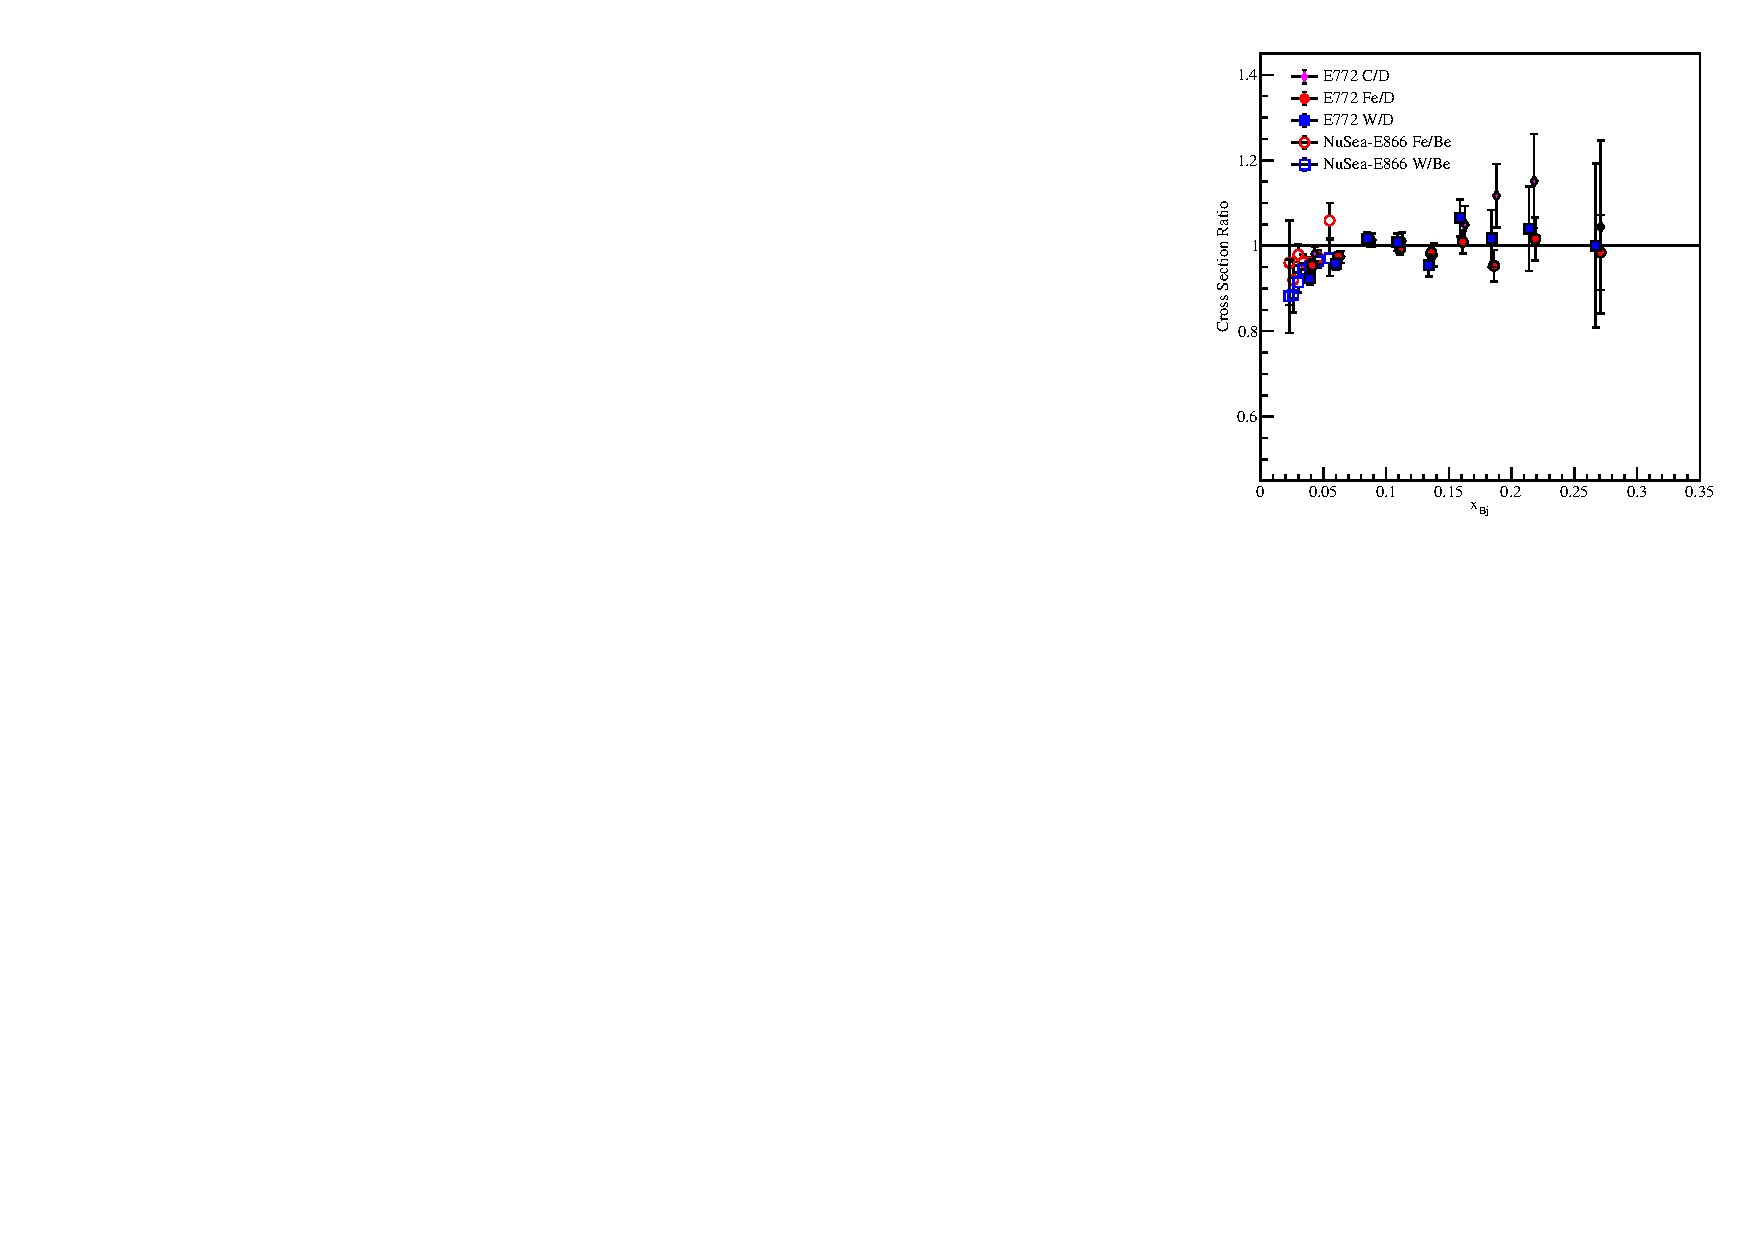
\includegraphics[width=0.45\textwidth]{plots/Drell-Yan_EMC.pdf}
  \caption{Drell-Yan cross section ratios from E772 and E866 \cite{Alde:1990im, Vasilev:1999fa}.}
  \label{fig:drell-yan}
\end{figure}
\end{center}


All these experiments use proton beams. They are mainly sensitive to the antiquark 
distributions in nuclei.  Since pions contain also valence antiquarks, pion beams are  
an ideal tool for the investigation of the valence quark distributions. Pion-induced Drell-Yan data have 
been taken in the past by two CERN experiments, NA3~\cite{Badier:1981ci} 
and NA10~\cite{Bordalo:1987cs}.  For both experiments the achieved statistics is limited
and the conclusions of the authors inconsistent.  

A dedicated Drell-Yan experiment, 
combining nuclear and deuterium targets could significantly improve the results. 
A high-intensity pion beam with incident momenta between 100 and 200 GeV/$c$ is presently available 
only at CERN. Since in Drell-Yan experiments the total cross section increases with the energy, a higher 
energy is preferable. On the other hand, a maximal coverage of the high-$x$ EMC could require a 
lower incident momentum.  

\subsubsection{Flavor dependence of the EMC effect} 
%The flavor dependence of the nuclear mean field was recently investigated~\cite{Cloet:2009qs} using a 
%covariant Nambu-Jona-Lasinio (NJL) model.  The main conclusion of this study is that for nuclei with 
%N$>$Z, the isovector-vector mean field affects differently the two lightest quark distributions,
%causing an additional attraction (repulsion) for the $u$ and $d$ quarks respectively. 
%This additional vector field modifies differently the corresponding nuclear PDFs, resulting in an effect of 
%the medium which is more than twice larger for the $u$ quarks. An experimental evidence of this flavor 
%dependence is still missing. 

The sensitivity of the available Drell-Yan data on the flavor-dependent effect was explored in 
Ref.~\cite{Dutta:2010pg}. A comparison with calculations based on the model of Ref.~\cite{Cloet:2009qs} 
shows that the  statistics of the available data~\cite{Badier:1981ci,Bordalo:1987cs} is insufficient to draw firm conclusions. 
The flavor dependence may also have an effect 
on the global nuclear PDF fits presently available. Indeed, when releasing the flavor constraints in these fits, 
the model uncertainties increase~\cite{Paakinen:2017} by a large factor. 

The effect coming fome the flavor dependence of the mean field can be further amplified by 
comparing positive and negative pion beam Drell-Yan data on the same heavy target. Negative pions probe mainly the 
target $u$-valence quarks, whereas positive pions prefer $d$-valence quarks. Pion beams of both charges
are presently available only at CERN. 

 \subsubsection{Nuclear dependence of the gluon distribution}

The effect of the nuclear mean field on the gluon distribution is presently unknown. Available nuclear PDFs produce 
very different results~\cite{Cazaroto:2008qh} in the whole region of $x$ and particularly for $x > 0.1$.
The J/$\psi$ production data, 
usually collected in parallel with Drell-Yan data, can be used as a probe of the nuclear gluon distributions. 
The production of J/$\psi$ proceeds through either the $q\bar q$ or the $gg$ fusion processes, the $gg$ 
contribution being the dominant one~\cite{Vogt:1999dw} for $x_F < 0.5$  even at low center-of-mass energies. 

As for Drell-Yan, most of the J/$\psi$ production data were taken with proton beams. The nuclear dependence 
was primarily used for the evaluation of the absorption of the J/$\psi$ as a function of the atomic number. 
Pion-induced J/$\psi$ data have been taken by several experiments, but most of the time with a single target. 
A comparison of several nuclear targets (SI, Cu, W) was also made~\cite{Alexandrov:1999ch},  
but unfortunately for the total cross-sections only. High-statistics J/$\psi$ production data on   
the $x$ dependence, combining nuclear and light targets, are still missing. 

The strong-interaction J/$\psi$ production process has one important advantage: its cross-section is large, 
Large statistics J/$\psi$ production data can be collected and 
used to precisely map out the $x$-dependence of the nuclear modifications. Such data could be 
used for a better assessment of the charmonium production process.  The gluon distributions could 
therefore be inferred with minimized model-dependence uncertainties.  

